\documentclass[10pt,letterpaper,oneside]{article}
\usepackage[margin=2.5cm]{geometry}
\usepackage[utf8]{inputenc}
\usepackage[francais]{babel}
\usepackage{amsmath}
\usepackage{amsthm}
\usepackage{amsfonts}
\usepackage{amssymb}
\usepackage{graphicx}
\usepackage{tikz}
\usetikzlibrary{decorations.pathreplacing,angles,quotes}

%Code
\usepackage{listings}
\lstset{
    literate={é}{{\'e}}1
    {è}{{\`e}}1
    {ê}{{\^e}}1
    {î}{{\^i}}1
    {à}{{\`a}}1
    {É}{{\'E}}1,
    basicstyle=\footnotesize\ttfamily,
    keywordstyle=\bfseries\color{green!70!black},
    identifierstyle=\color{blue},
    commentstyle=\ttfamily\color{red!70!black}\emph,
    stringstyle=\bfseries\color{orange},
    showstringspaces=false,
    language=python,
    breaklines=true
}

% Algorithmes
\usepackage{algpseudocode}
\usepackage{algorithm}
\floatname{algorithm}{Algorithme}
\algrenewcommand\algorithmicwhile{\textbf{tant que}}
\algrenewcommand\algorithmicfunction{\textbf{fonction}}
\algrenewcommand\algorithmicend{\textbf{fin}}
\algrenewcommand\algorithmicdo{\textbf{faire}}
\algrenewcommand\algorithmicfor{\textbf{pour}}
\algrenewcommand\algorithmicif{\textbf{si}}
\algrenewcommand\algorithmicelse{\textbf{sinon}}
\algrenewcommand\algorithmicthen{\textbf{alors}}
\algrenewcommand\algorithmicreturn{\textbf{retourner}}
\algrenewcommand\algorithmicrepeat{\textbf{faire}}
\algrenewcommand\algorithmicuntil{\textbf{tant que}}
\newcommand{\enteteproc}[2]{\vskip\baselineskip \hspace*{\fill} \algorithmicprocedure~\Call{#1}{#2} \hspace*{\fill} \vskip\baselineskip}
\newcommand{\entetefunc}[3]{\vskip\baselineskip \hspace*{\fill} \algorithmicfunction~\Call{#1}{#2} : #3 \hspace*{\fill} \vskip\baselineskip}
\newcommand{\algorithmicbreak}{\textbf{arrêt}}
\newcommand{\Break}{\State \algorithmicbreak}

\usepackage{xargs}
\usepackage{xcolor}
\usepackage[colorinlistoftodos,prependcaption,textsize=tiny]{todonotes}
\newcommandx{\emile}[2][1=]{\todo[linecolor=green,backgroundcolor=green!25,bordercolor=green,#1]{#2}}

\newtheorem{definition}{Définition}
\newtheorem{lemme}{Lemme}
\newtheorem{proposition}{Proposition}
\newtheorem{theorem}{Théorème}

\newcommand{\bigo}{\mathcal{O}}

\author{Émile Nadeau, NADE10059404}
\title{Identification du vocabulaire des carrés en temps linéaire \\ \small Rapport remis dans le cadre du cours Algèbre Computationnelle}
\begin{document}
    \maketitle
    \section{Introduction et définitions}
    Un carré, est une mot $\alpha\alpha$ où $\alpha$ est non vide. On s'intéresse ici au repérage des carrés dans un mot $S=s_0s_1\cdots s_{n-1}$  donné et de longueur $n$ sur un alphabet $\Sigma$ de taille finie. On note $S[i]:=s_i$ et $S[i:j]:=s_is_{i+1}\cdots s{j-1}$.
    \begin{definition}
        Deux carrés $\alpha\alpha$ et $\alpha'\alpha'$ sont de \emph{types} différents si $\alpha\neq \alpha'$.
    \end{definition}
    \begin{definition}
        Soit $w$ un mot. Le \emph{vocabulaire des carrés} de $w$ est l'ensemble des types de carré qui apparaisse dans $w$.
    \end{definition}
    Pour des raisons de simplicité, on référera simplement au \emph{vocabulaire} du mot.  En 1998, Fraenkel et Simpson démontre dans \cite{MR1616571} que la taille du vocabulaire est linéaire en la taille du mot. Plus précisément, ils démontrent le théorème suivant:
    \begin{theorem} \label{thm:bornecarre}
        Soit $S$ un mot de longueur $n$. Pour chaque position $i$ dans $S$, il y a au plus deux types de carrés dont l'occurrence la plus à droite commence à $i$.
        En particulier, a taille du vocabulaire de $S$ est bornée par $2n$.
    \end{theorem}
    La question naturelle qui survient lorsqu'on sait que la taille du vocabulaire est en $\bigo(n)$ est de savoir s'il est possible de trouver une occurrence du type de chaque carré d'un mot en $\bigo(n)$. La solution à ce problème est présentée par Gusfield et Stoye pour un alphabet fini de taille fixée dans \cite{MR2096375}. Nous présenterons ici leurs résultats et une implémentation de leur algorithme.  L'algorithme se décompose en trois phases qui s'effectuent toutes en temps et espace linéaire.
    
    Pour leur algorithme, ils utilisent l'arbre suffixe à la fois comme outil de calcul et comme support pour le résultat de l'algorithme. Commençons donc par quelques rappels sur l'arbre suffixe.
    
    \subsection{Arbres suffixes}
    L'arbre suffixe de $S$, noté $T(S)$,  est une compactification de la trie suffixe de $S$, cette dernière étant l'automate déterministe en forme d'arbre reconnaissant tous les suffixes de $S$. L'arbre suffixe peut être construit et stocké en $\bigo(n)$ comme démontré par Ukkonen dans \cite{MR1343552}. Toutefois, avec l'algorithme de construction de Ukkonen et implémenté dans Sage, un suffixe n'est pas forcément associé à une feuille dans $T$. Pour expliciter tous les états finaux, on ajoute à la fin du mot un symbole \$ qui n'apparaît nul part ailleurs dans le mot. On trouve en Annexe~\ref{ann:arbre} un exemple d'arbre suffixe.
    
    On dira qu'un nœud $v$ de l'arbre suffixe à une \emph{étiquette de chemin} $L(v)$ si la lecture des arêtes de la racine au noeud $v$ donne le mot $L(v)$. Par exemple, le noeud 5 dans l'exemple de l'Annexe~\ref{ann:arbre} à une étiquette de chemin $L(5)=abaab$. On note $D(v)=|L(v)|$ la \emph{profondeur de mot} du noeud $v$. Le noeud 5 dans notre exemple a donc une profondeur de mot $D(5)=5$.
    
    On peut lire tous les facteurs d'un mot dans l'arbre suffixe car on peut y lire tous les suffixes et un facteur est forcément préfixe d'un certain suffixe. Pour marquer un facteur particulier dans l'arbre suffixe, on enregistre le point où il se termine  lorsqu'on le lit à partir de la racine. Pour retrouver ce facteur, il suffit alors de lire les arêtes sur le chemin de la racine au point qui est marqué. Précisément, si la lecture d'un facteur s'arête après avoir lu $\ell$ lettres sur une arête $(u,v)$ alors on note le point final $((u,v),\ell)$. On note que $1\leq \ell \leq D(v)-D(u)$ car si on veut indiquer que la lecture s'arrête à $u$, on prendra l'arête entrante de $u$ et que le nombre de lettre lues sur $(u,v)$ ne peut pas excéder le nombre à ajouter pour passer de $L(u)$ à $L(v)$.
    
    Le \emph{lien suffixe} d'un noeud $v$ avec étiquette de chemin $aw$ ($a$ une lettre, $w$ un mot) est défini comme $f(v)=v'$ avec $v'$ tel que $L(v')=w$. Le lien suffixe fait partie de la structure de données d'arbre suffixe et est calculé durant la construction. Par la suite, le calcul du lien suffixe d'un noeud ce fait en temps constant.
    
    On a aussi que chaque position dans $S$ est associée avec la feuille du suffixe commençant à cette position. Cette association peut être calculée en temps linéaire par un parcours de l'arbre.
    
    \subsection{Relation de couverture} \label{sec:couverture}
    On identifiera une occurrence d'un type de carré par une paire $(i,l)$ où $i$ indique la position de départ du carré dans le mot et $l$ la longueur du carré. Dans $S$ la paire $(i,l)$ indique donc le facteur $s_is_{i+1}\cdots s_{i+l-1}$. Le vocabulaire peut alors être représenté par un ensemble de paires $(i,l)$ spécifiant chacune une occurrence d'un type différent de carré du vocabulaire. Pour $w$ un mot et $a$ une lettre, on dit que $wa$ est la \emph{rotation à droite} de $aw$.
    \begin{definition}
        On dit $i,i+1,\dots,j-1,j$ forme une \emph{$l$-série} de carrés si $(i,l)$, $(i+1,l)$, \dots, $(j,l)$ sont tous des carrés.
    \end{definition}
    Par exemple, dans $aabaabaaa\$$ les positions $0,1,2$ forme une $6$-série.
    \begin{definition}
        On dit qu'un carré $(i,l)$ \emph{couvre} un carré $(j,l)$ si $i,i+1,\dots, j$ forme une $l$-série.
        On dit qu'un ensemble de paire est un \emph{ensemble couvrant} si au moins une occurrence de chaque carré du vocabulaire est couverte par une paire dans l'ensemble.
        Si l'occurrence la plus à gauche de chaque carré du vocabulaire est couverte par une paire de l'ensemble couvrant on dira alors que c'est un \emph{ensemble couvrant le plus à gauche}.
    \end{definition}
    Si on reprend l'exemple $abaabaabbaaabaaba\$$ on a que
    $(0,6)$ couvre $(2,6)$ car $0,1,2$ forme une $6$-série.
     Dans notre exemple, le vocabulaire est
    $\{aa,bb,aabaab,abaaba,baabaa\}$
    donc $\{(0,6),(7,2),(10,2)\}$ forme un ensemble couvrant mais pas le plus à gauche alors que
    $\{(0,6),(2,2),(8,2)\}$ est un ensemble couvrant le plus à gauche.
    \section{Algorihtmes préliminaires}
    \subsection{Décomposition de Lempel-Ziv}
    La \emph{décomposition de Lempel-Ziv}  une factorisation d'un mot $S=s_0s_1\cdots  s_{n-1}$ en facteur $S[i_B:i_{B+1}]$ où $i_B$ est définie récursivement comme $i_1=1$ et $i_{B+1}=i_B+\max(1,l_{i_B})$ avec $l_k$ indiquant la longueur du plus long préfixe de $s_k\cdots s_{n-1}$ qui a une occurrence dans $S$ qui commence avant $s_k$. On appel ces facteurs des \emph{blocs}.

    Pour construire la décomposition, on note d'abord que le premier bloc est la première lettre car clairement, $l_0=0$. Ensuite, pour trouver le bloc suivant, on considère la position $k$ suivant le dernier bloc construit. Si on a la première apparition d'une lettre alors on a un bloc de longueur 1 (la lettre seulement) car $l_k$ est nul. Si la lettre est déjà apparu alors $l_k\geq 1$ et donc le bloc débutant à cette lettre sera le plus long facteur commençant à cette position qui a une occurrence dans $S$ débutant avant cette position.
    
    On peut construire cette décomposition en temps linéaire à partir de l'arbre suffixe. Pour ce faire, on utilise la propriété que les étiquettes des arcs de l'arbre indique la première apparition de ce facteur. Plus précisément, si on a un facteur du mot dont la lecture s'arrête sur une arête d'étiquette $(i,j)$ alors la dernière lettre de la première apparition de ce facteur est entre $i$ et $j-1$. 
    Pour trouver le plus long facteur commençant à une certaine position dans $S$ et ayant une occurrence commençant avant, on peut donc lire le facteur dans l'arbre suffixe et s'arrêter lorsqu'on dépasse la fin du facteur qu'on est entrain de lire. 
    
    Pour clarifier, voici une exemple avec le mot \emph{cacao} (voir Figure~\ref{fig:caco_suffix_tree}).
    On cherche le plus long facteur qui commence à la position 2. À cette position, ce trouve un \emph{c} on suit donc la \emph{c}-transition à partir de la racine qui est l'arête $(0,2)$. On a donc une apparition du facteur \emph{ca} avant celle commençant en position 2. Après \emph{ca} la prochaine lettre est \emph{o}. La \emph{o}-transition à partir l'état 3 est l'arête $(4,5)$ on s'arrête donc  car le premier facteur cao se termine en 4 et est donc celui commençant en 2.
    
    \begin{figure}[htb]
        \centering
        %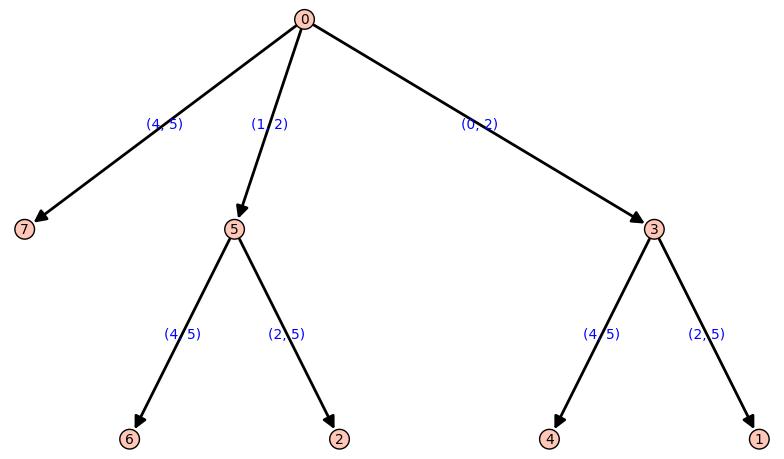
\includegraphics[width=10cm]{figure/cacao_suffix_tree.png}
        \begin{tikzpicture}[>=latex,line join=bevel,]
%%
\node (node_7) at (177.0bp,77.5bp) [draw,draw=none] {$7$};
  \node (node_6) at (177.0bp,6.5bp) [draw,draw=none] {$6$};
  \node (node_5) at (120.0bp,77.5bp) [draw,draw=none] {$5$};
  \node (node_4) at (63.0bp,6.5bp) [draw,draw=none] {$4$};
  \node (node_3) at (63.0bp,77.5bp) [draw,draw=none] {$3$};
  \node (node_2) at (120.0bp,6.5bp) [draw,draw=none] {$2$};
  \node (node_1) at (6.0bp,6.5bp) [draw,draw=none] {$1$};
  \node (node_0) at (120.0bp,148.5bp) [draw,draw=none] {$0$};
  \draw [red,->] (node_0) ..controls (105.5bp,141.6bp) and (90.86bp,134.39bp)  .. (82.0bp,124.0bp) .. controls (74.654bp,115.39bp) and (69.827bp,103.53bp)  .. (node_3);
  \definecolor{strokecol}{rgb}{0.0,0.0,0.0};
  \pgfsetstrokecolor{strokecol}
  \draw (99.0bp,113.0bp) node {$\left(0, 2\right)$};
  \draw [red,->] (node_3) ..controls (48.498bp,70.599bp) and (33.86bp,63.386bp)  .. (25.0bp,53.0bp) .. controls (17.654bp,44.388bp) and (12.827bp,32.533bp)  .. (node_1);
  \draw (42.0bp,42.0bp) node {$\left(2, 5\right)$};
  \draw [red,->] (node_5) ..controls (120.0bp,60.331bp) and (120.0bp,38.741bp)  .. (node_2);
  \draw (137.0bp,42.0bp) node {$\left(2, 5\right)$};
  \draw [blue,->] (node_0) ..controls (120.0bp,131.33bp) and (120.0bp,109.74bp)  .. (node_5);
  \draw (137.0bp,113.0bp) node {$\left(1, 2\right)$};
  \draw [green,->] (node_0) ..controls (133.78bp,140.85bp) and (146.75bp,133.51bp)  .. (155.0bp,124.0bp) .. controls (162.69bp,115.14bp) and (168.35bp,103.13bp)  .. (node_7);
  \draw (185.0bp,113.0bp) node {$\left(4, 5\right)$};
  \draw [green,->] (node_3) ..controls (63.0bp,60.331bp) and (63.0bp,38.741bp)  .. (node_4);
  \draw (80.0bp,42.0bp) node {$\left(4, 5\right)$};
  \draw [green,->] (node_5) ..controls (133.78bp,69.847bp) and (146.75bp,62.506bp)  .. (155.0bp,53.0bp) .. controls (162.69bp,44.142bp) and (168.35bp,32.128bp)  .. (node_6);
  \draw (185.0bp,42.0bp) node {$\left(4, 5\right)$};
%
\end{tikzpicture}

        \caption{Arbre suffixe de cacao}\label{fig:caco_suffix_tree}
    \end{figure}

La méthode détaillée pour calculer la décomposition est décrite dans l'Algorithme~\ref{alg:LZ-decomposition}. On se convainc facilement que cet algorithme a une complexité en $\bigo(n)$ où $n$ est la longueur du mot. En effet, chaque instruction s'effectue en temps constant (on suppose que la taille de l'alphabet est finie) et les boucles n'ont pour effet que de lire une seule fois $S$.
\begin{algorithm}
\caption{Décomposition de Lempel-Ziv}
\label{alg:LZ-decomposition}
\begin{algorithmic}[1]
    \Function{LZ-decomposition}{T: arbre suffixe}: liste d'entier
        \State blocs $\gets [0]$
        \State $i\gets 0$
        \State $S\gets T.\Call{mot}$
        \While{$i<|S|$}
            \State $l\gets 0$
            \State Soit $(x,y)$ la $S[i]$-transition à partir de la racine de $T$
            \While{$x<i+l$}
                \If{$y=|S|$}
                    \State $l\gets |S|-i$
                \Else
                    \State $l\gets l+y-x$
                \EndIf
                \If{$i+l\geq|S|$}
                    \State $l\gets |S|-i$
                    \Break
                \EndIf
                \State Soit $(x,y)$ la $S[i+l]$-transition à partir de l'extrémité de $(x,y)$
            \EndWhile
            \State blocs.$\Call{ajouter}{\max(l,1)}$
        \EndWhile
    \EndFunction
\end{algorithmic}
\end{algorithm}
\subsection{Plus longues extensions communes vers l'avant et l'arrière}
Un autre sous-problème à résoudre est le calcul des plus longues extensions vers l'avant et vers l'arrière dans un mot. Ce problème consiste, étant donné deux positions $i$ et $j$ dans $S$, à trouver le plus long facteur commun commençant (resp. terminant) à $i$ et $j$. On nomme ce facteur \emph{plus longue extension commune vers l'avant} (resp. \emph{vers l'arrière}). Par exemple dans le mot $aabaabaa$ pour les position 1 et 4  la plus longue extension commune est $abaa$ vers l'avant et $aa$ vers l'arrière.

On présente ici le traitement du problème de plus longue extension commune vers l'avant puisque pour celle vers l'arrière il suffit de considérer le mot à l'envers. Dans le chapitre de 8 de \cite{MR1460730}, Gusfield présente un algorithme qui permet après un prétraitement en $\bigo(n)$ de retrouver le plus petit ancêtre commun de n'importe quelle paire de nœud dans un arbre en temps constant.

Dans notre cas précis, le prétraitement s'effectue en deux partie On doit prétraiter l'arbre suffixe pour le calcul du plus petit ancêtre commun. Par un simple parcours, on crée aussi une association qui permet en temps constant de trouver $D(v)$ pour tout nœud $v$. L'Algorithme~\ref{alg:LCE} permet alors de retrouver en temps constant la longueur de la plus longue extension commune en temps constant.

\begin{algorithm}[htb]
    \caption{Calcul de la plus longue extension commune}
    \label{alg:LCE}
    \begin{algorithmic}[1]
        \Function{LCE}{i,j: position}: entier
            \State $v_1\gets $ la feuille associée au suffixe commençant en position $i$
            \State $v_2\gets $ la feuille associée au suffixe commençant en position $j$
            \State $v\gets  \Call{plusPetitAncêtreCommun}{v_1,v_2}$
            \State \Return $D(v)$
        \EndFunction
    \end{algorithmic}
\end{algorithm}

Pour l'implémentation, j'ai toutefois choisi l'approche naïve qui consiste à comparer caractère par caractère les chaînes démarrant aux positions $i$ et $j$  jusqu'à trouver une différence (voir Algorithme~\ref{alg:LCEnaive})

\begin{algorithm}[htb]
    \caption{Calcul de la plus longue extension commune (approche naïve)}
    \label{alg:LCEnaive}
    \begin{algorithmic}[1]
        \Function{LCE}{$S$:mots, $i,j$: positions}: entier
            \State $l\gets 0$
            \While{$S[i+l]=S[j+l]$}
                \State $l\gets l+1$
            \EndWhile
            \Return $l$
        \EndFunction
    \end{algorithmic}
\end{algorithm}

Le choix de cette approche plus simple est justifié par les résultats de Ilie, Navarro et Tinta qui dans \cite{MR2735498} démontre que l'approche naïve est plus efficace en moyenne et plus rapide en pratique. L'intérêt de cette méthode est aussi sa simplicité d'implémentation.

\subsection{Stratégie compter et sauter} \label{sec:count&skip}
Dans un arbre suffixe, la stratégie compter et sauter est une façon accélérée de lire un facteur à partir d'un nœud si on sait à l'avance qu'on peut lire ce facteur à partir de ce noeud. La stratégie est la suivante, si on veut lire le facteur $s_is_{i+1}\cdots s_{j-1}$ à partir du noeud $u$. On regarde la $s_i$ transition à partir de $u$ et si le facteur associé à l'arête est moins long que la longueur du facteur à lire, on saute l'arête et on répète avec le prochain noeud et le reste du facteur à lire. Si on veut lire le facteur $s_is_{i+1}\cdots s_{j-1}$ dans $T(S)$ à partir du noeud $u$, la façon de faire est alors décrite par l'Algorithme~\ref{alg:coutn&skip}.

\begin{algorithm}[htb]
    \caption{Stratégie compter et sauter}
    \label{alg:coutn&skip}
    \begin{algorithmic}[1]
        \Function{compterEtSauter}{$u$: noeud, $i,j$: positions}: entier
            \State Soit $(u,v)$ l'arête de la $s_i$-transition de $u$
            \State $l\gets D(v)-D(u)$
            \If {$l\geq j-i$}
                \State \Return $((u,v),j-i)$
            \EndIf
            \State \Return $\Call{CompterEtSauter}{v,i+l,j}$
        \EndFunction
    \end{algorithmic}
\end{algorithm}

Cette stratégie permet de sauter chaque arête en temps constant et d'avoir une complexité au pire cas en $O(j-i)$ alors que tous les cas on une complexité en $\Theta(j-i)$ si on lit le facteur au complet.

\section{Phase I:~Trouver un ensemble couvrant le plus à gauche}

L'objectif de cette phase est de construire en temps linéaire un ensemble couvrant le plus à gauche comme décrit dans la Section~\ref{sec:couverture}. Pour ce faire, on utilisera la décomposition de Lempel-Ziv. On commence donc par quelques résultats sur  le liens entre les positions des occurrences les plus à gauche des carrés et les blocs.

\begin{lemme} \label{lem:seconde_moitie}
    La seconde moitié d'un carré $\alpha\alpha$ d'un mot $S$ doit toucher au plus deux blocs de la décomposition de Lempel-Ziv de $S$.
\end{lemme}

\begin{proof}
    Supposons que la seconde moitié $\alpha$ touche plus de deux bloc. Soit $\beta$ le premier bloc complètement inclus dans $\alpha$ et $\eta$ le suffixe de $\alpha$ suivant $\beta$. Alors $\eta$ est forcément non-vide car le $\alpha$ de droite touche au moins trois blocs. Comme $\alpha\alpha$ est un carré, il y a une occurrence précédente de $\beta\eta$ dans $S$  ce qui contredit que le bloc $\beta$ est de longueur maximale.
\end{proof}

\begin{lemme} \label{lem:touche2}
    L'occurence la plus à gauche d'un carré dans $S$ touche au moins deux blocs de la décomposition de Lempel-Ziv de $S$.
\end{lemme}

\begin{proof}
    Supposons que la première apparition d'un carré apparaisse complètement dans un bloc $\beta$. Alors par définition de la décomposition, $\beta$ a une occurrence plus à gauche dans le mot et donc le carré aussi.
\end{proof}

On appel \emph{centre} d'un carré $\alpha\alpha$ la dernière lettre de la première moitié. On alors le théorème suivant où le bloc $B$ est le bloc $S[i_B:i_{B+1}]$.

\begin{theorem} \label{thm:conditioncarre}
    Si la première occurrence (la plus à gauche) d'un carré $\alpha\alpha$ a son centre dans un bloc $B$ alors soit
    \begin{itemize}
        \item (Condition~1) $\alpha\alpha$ a son début  à l'intérieur du bloc $B$ et sa fin dans le bloc $B+1$;
        
        ou
        \item (Condition~2) $\alpha\alpha$ a son début dans le bloc $B-1$ ou avant et sa fin dans le bloc $B$ ou $B+1$.
    \end{itemize}
\end{theorem}
\begin{proof}
    Soit $\alpha\alpha$ un carré ayant son centre dans le bloc $B$. Supposons que $\alpha\alpha$ ne satisfassent pas la condition 1. Alors ou bien son début est avant le bloc $B$ ou bien sa fin n'est pas dans le bloc $B+1$.

    Si son début n'est pas dans le bloc $B$ alors il est dans le bloc $B-1$ ou avant. Si son centre est le dernier caractère du bloc $B$ alors le bloc $B+1$ a $\alpha$ comme préfixe car on sait que $\alpha$ a une occurrence plus à droite dans la chaîne. On a donc que le dernier caractère du carré est dans $B+1$. Si le centre n'est pas le dernier caractère de $B$ alors la fin du carré est dans $B+1$ car la seconde moitié ne peut toucher plus de deux blocs (Lemme~\ref{lem:seconde_moitie}).

    Si sa fin n'est pas dans le bloc $B+1$, elle doit être dans le bloc $B$.
    En effet, le centre ne peut pas être la dernière lettre du bloc $B$ car alors le bloc $B+1$ aurait $\alpha$ comme préfixe et la fin de l'occurrence serait donc dans $B+1$.
    La fin doit donc être dans $B$ car la seconde moitié d'un carré touche $B$ et ne peut pas toucher plus de deux bloc (Lemme~\ref{lem:seconde_moitie}). De plus, la première occurrence d'un carré doit toucher au moins deux blocs par le Lemme~\ref{lem:touche2} et donc le début doit être dans le bloc $B-1$ ou avant.
\end{proof}

On dit qu'un carré est de  \emph{type~1} (resp. \emph{type~2}) si il satisfait la condition~1 (resp. condition~2) du théorème. Pour chacune des conditions du théorème précédent, on présente ici l'Algorithme~\ref{alg:leftmostcovering} qui maintient l'invariant suivant: Après avoir traité les blocs $1,2,3,...,B$ toutes les occurrences les plus à gauches de carrés qui ont leur centre dans les blocs $1,2,3,...,B$ sont couvertes par une des paires engendrées par l'algorithme. Pour pouvoir compléter la preuve des résultat de \cite{MR2096375}, il faut toutefois noter qu'il y a trois petites erreurs à corriger dans l'algorithme. Pour le type~1, il faut ajouter la condition $start\geq h$ pour le si. Pour le type~2, il faut prendre $k$ seulement à partir de $2$ et changer $start+k<h_1$ pour $start+k\leq h_1$
\begin{algorithm}[htb]
    \centering
    \caption{Traitement du bloc $B$ pour l'ensemble couvrant le plus à gauche}
    \label{alg:leftmostcovering}
    \vspace{10pt}
    \begin{algorithmic}[1]
        \State Soit $h$ le point de départ de $B$
        \State Soit $h_1$ le point de départ de $B+1$
        \Function {carrésType1}{ } : paires de carrés
            \For{$k=1,2...,|B|$}
                \State $q\gets h_1-k$
                \State $k_1\gets$ longueur de la plus longue extension commune vers l'avant commencant à $h_1$ et $q$
                \State $k_2\gets$ longueur de la plus longue extension commune vers l'arrière commencant à $h_1-1$ et $q-1$
                \State start$\gets \max(q-k_2,q-k+1)$
                \If{$(k_1+k_2\geq k) \wedge (k_1>0) \wedge (start\geq h)$}
                    \State \textbf{engendrer} (start,$2k$)
                \EndIf
            \EndFor
        \EndFunction
        \State
        \Function{carrésType2}{ }: paires de carrés
            \State Soit $B$
            \For{$k=2,3...,|B|+|B+1|$}
                \State $q\gets h+k$
                \State $k_1\gets$ longueur de la plus longue extension commune vers l'avant commencant à $h$ et $q$
                \State $k_2\gets$ longueur de la plus longue extension commune vers l'arrière commencant à $h_1-1$ et $q-1$
                \State start$\gets \max(h-k_2,h-k+1)$
                    \If{$(k_1+k_2\geq k) \wedge (k_1>0) \wedge (start+k\leq h_1) \wedge (k_2>0)$}
                        \State \textbf{engendrer} (start,$2k$)
                    \EndIf
            \EndFor
        \EndFunction
    \end{algorithmic}
\end{algorithm}

\begin{lemme}
    Toutes les paires retournées par l'Algorithme~\ref{alg:leftmostcovering} représentent des carrés.
\end{lemme}

\begin{proof}
    Regardons d'abord le type~1. Si une paire est retournée alors $k_1+k_2\geq  k$ et on peut décomposer le mot comme illustré à la Figure~\ref{fig:phase1a}. On a alors que $q-k_2$ indique le début du premier facteur $\alpha$ et donc $(q-k_2,2k)$ est bien un carré puisqu'il indique $(tuv)^2$. Si $q-k+1$ est plus grand que $q-k_2$ alors $k_2\geq k$ et la définition de $k_2$ nous donne donc
    $$S[q:h_1]=S[h_1-k:h_1]=S[q-k:q]$$
    De plus, si une paire est retournée $k_1>0$ donc $S[h_1]=S[q]$. Ainsi, $S[q+1:h_1+1]=S[q-k+1:q+1]$
    Donc $(q-k+1,2k)$ est le carré $S[q-k+1:h_1+1]$.
    \begin{figure}[htb]
        \centering
        \begin{tikzpicture}[scale=0.5]
    %Boite supérieur et indice
    \draw (-2,0)--(17,0);
    \draw (-2,1)--(17,1);
    \draw (-1,1)--(-1,0);
    \draw (13,1)--(13,0);
    \node at (-2,0.5) {$\dots$};
    \node at (16,0.5) {$\dots$};
    \node[above right] at (-1,1) {$h$};
    \node[above right] at (13,1) {$h_1$};
    \node[above] at (8,1) {$q$};
    \draw[decoration={brace,raise=5pt},decorate]
    (8,1.5) -- node[above=6pt] {$k$} (13,1.5);
    %Flèche pour $k_i$
    \draw[->] (13,0.85)--(9.5,0.85);
    \node[below] at (12,1) {\scriptsize $k_2$};
    \draw[->] (8,0.85)--(4.5,0.85);
    \node[below] at (6,1) {\scriptsize $k_2$};
    \draw[->] (13,0.15)--(15.5,0.15);
    \node[above] at (9,0) {\scriptsize $k_1$};
    \draw[->] (8,0.15)--(10.5,0.15);
    \node[above] at (14,0) {\scriptsize $k_1$};
    %Facteur alpha beta
    \draw (13,-1) rectangle (9.5,-2) node[pos=.5] {$\alpha$};
    \draw (8,-2) rectangle (4.5,-3) node[pos=.5] {$\alpha$};
    \draw (13,-1) rectangle (15.5,-2) node[pos=.5] {$\beta$};
    \draw (8,-2) rectangle (10.5,-3) node[pos=.5] {$\beta$};
    %Facteur w,u,t
    \draw (10.5,-3) rectangle (9.5,-4) node[pos=.5] {$t$};
    \draw (10.5,-3) rectangle (13,-4) node[pos=.5] {$u$};
    \draw (8,-3) rectangle (9.5,-4) node[pos=.5] {$v$};
    \draw (4.5,-3) rectangle (5.5,-4) node[pos=.5] {$t$};
    \draw (8,-3) rectangle (5.5,-4) node[pos=.5] {$u$};
    \draw (13,-3) rectangle (14.5,-4) node[pos=.5] {$v$};
    \draw (14.5,-3) rectangle (15.5,-4) node[pos=.5] {$t$};
\end{tikzpicture}
        \caption{Algorithme~\ref{alg:leftmostcovering} pour le type~1 avec $k_1+k_2\geq k$} \label{fig:phase1a}
    \end{figure}
    
    Dans le cas du type~2 la preuve est similaire au type~1 mais $h$ joue le rôle qu'avait $q$ et $q$ le rôle qu'avait $h_1$ (voir Figure~\ref{fig:phase1b}).
    \begin{figure}[htb]
        \centering
        \begin{tikzpicture}[scale=0.5]
    %Boite supérieur et indice
    \draw (3,0)--(17,0);
    \draw (3,1)--(17,1);
    \draw (8,1)--(8,0);
    \node at (3,0.5) {$\dots$};
    \node at (16,0.5) {$\dots$};
    \node[above right] at (13,1) {$q$};
    \node[above] at (8,1) {$h$};
    \draw[decoration={brace,raise=5pt},decorate]
    (8,1.5) -- node[above=6pt] {$k$} (13,1.5);
    %Flèche pour $k_i$
    \draw[->] (13,0.85)--(9.5,0.85);
    \node[below] at (12,1) {\scriptsize $k_2$};
    \draw[->] (8,0.85)--(4.5,0.85);
    \node[below] at (6,1) {\scriptsize $k_2$};
    \draw[->] (13,0.15)--(15.5,0.15);
    \node[above] at (9,0) {\scriptsize $k_1$};
    \draw[->] (8,0.15)--(10.5,0.15);
    \node[above] at (14,0) {\scriptsize $k_1$};
%    %Facteur alpha beta
%    \draw (13,-1) rectangle (9.5,-2) node[pos=.5] {$\alpha$};
%    \draw (8,-2) rectangle (4.5,-3) node[pos=.5] {$\alpha$};
%    \draw (13,-1) rectangle (15.5,-2) node[pos=.5] {$\beta$};
%    \draw (8,-2) rectangle (10.5,-3) node[pos=.5] {$\beta$};
%    %Facteur w,u,t
%    \draw (10.5,-3) rectangle (9.5,-4) node[pos=.5] {$t$};
%    \draw (10.5,-3) rectangle (13,-4) node[pos=.5] {$u$};
%    \draw (8,-3) rectangle (9.5,-4) node[pos=.5] {$v$};
%    \draw (4.5,-3) rectangle (5.5,-4) node[pos=.5] {$t$};
%    \draw (8,-3) rectangle (5.5,-4) node[pos=.5] {$u$};
%    \draw (13,-3) rectangle (14.5,-4) node[pos=.5] {$v$};
%    \draw (14.5,-3) rectangle (15.5,-4) node[pos=.5] {$t$};
\end{tikzpicture}
        \caption{Algorithme~\ref{alg:leftmostcovering} pour le type~2 avec $k_1+k_2\geq k$} \label{fig:phase1b}
    \end{figure}
\end{proof}

\begin{lemme}\label{lem:couvre}
    Si $S$ possède deux carrés $(i,2k)$ et $(j,2k)$ tel que $i\leq j\leq i+k$ alors $(i,2k)$ couvre $(j,2k)$.
\end{lemme}

\begin{proof}
    Soit $\alpha\alpha$ et $\beta\beta$ ces carrés.
    Par les conditions sur $j$, les deux carrés ont une portion commune de longueur au moins $k$. On peut décomposer la portion couverte par $\alpha\alpha$ et $\beta\beta$ en facteur $u$ et $v$ comme à la Figure~\ref{fig:cover} de sorte que $|u|+|v|=k$.
    \begin{figure}[htb]
        \centering
        \begin{tikzpicture}[scale=0.5]
    %Facteur alpha beta, i,j
    \node[above] at (0,1) {$i$};
    \node[above] at (4,1) {$j$};
    \node[above] at (2,1) {$r$};
    \draw (0,0) rectangle (5,1) node[pos=.5] {$\alpha$};
    \draw (5,0) rectangle (10,1) node[pos=.5] {$\alpha$};
    \draw (4,0) rectangle (9,-1) node[pos=.5] {$\beta$};
    \draw (9,0) rectangle (14,-1) node[pos=.5] {$\beta$};
    %Facteur u,v,w
    \draw (0,-1) rectangle (4,-2) node[pos=.5] {$u$};
    \draw (4,-1) rectangle (5,-2) node[pos=.5] {$v$};
    \draw (5,-1) rectangle (9,-2) node[pos=.5] {$u$};
    \draw (9,-1) rectangle (10,-2) node[pos=.5] {$v$};
    \draw (10,-1) rectangle (14,-2) node[pos=.5] {$u$};
    %Mot intermédiaire
    \draw (2,-2) rectangle (7,-3) node[pos=.5] {$\gamma$};
    \draw (7,-2) rectangle (12,-3) node[pos=.5] {$\gamma'$};
    %Facteur u,v,w
    \draw (0,-3) rectangle (2,-4) node[pos=.5] {$u_1$};
    \draw (2,-3) rectangle (4,-4) node[pos=.5] {$u_2$};
    \draw (4,-3) rectangle (5,-4) node[pos=.5] {$v$};
    \draw (5,-3) rectangle (7,-4) node[pos=.5] {$u_1$};
    \draw (7,-3) rectangle (9,-4) node[pos=.5] {$u_2$};
    \draw (9,-3) rectangle (10,-4) node[pos=.5] {$v$};
    \draw (10,-3) rectangle (12,-4) node[pos=.5] {$u_1$};
    \draw (12,-3) rectangle (14,-4) node[pos=.5] {$u_2$};
\end{tikzpicture}
        \caption{$(i,2k)$ couvre $(j,2k)$} \label{fig:cover}
    \end{figure}
    Pour montrer que $(i,2k)$ couvre $(j,2k)$, il faut voir qu'on a une $2k$-série qui va de $i,i+1,\dots j$. Pour ce faire, on doit voir que $(r,2k)$ est un carré pour tout $i\leq r\leq j$. Soit $u_1$ le préfixe de longueur $r-i$ de $u$ et $u_2$ le suffixe correspondant. On a alors que $(r,2k)$ est le mot $(u_2vu_1)(u_2vu_1)$ qui est un carré.
\end{proof}

\begin{proposition} \label{prop:couvre}
    Soit $\gamma\gamma$ un carré de longueur $2k$ de $w$ qui satisfait la condition~1 ou la condition~2. Alors $\gamma\gamma$ est couvert par une des paires générées par l'Algorithme~\ref{alg:leftmostcovering}.
\end{proposition}

\begin{proof}
    Soit $c$ le centre de $\gamma\gamma$. Le carré est donc décrit par la paire $(c-k+1,2k)$. Soit $B$ le bloc contenant $c$ et $h$ le point de départ du bloc $B$. Soit $h_1$ le départ de $B+1$.
    
    \textbf{Si $(c-k+1,2k)$ satisfait la condition 2} alors sa fin est dans $B$ ou $B+1$ et donc $k\leq |B|+|B+1|$. De plus, son début est dans $B-1$ ou avant donc $k\geq 2$. Le carré devrait donc être couvert par \Call{carréType2}{} sur le bloc $B$ avec $k$.  Comme son début est dans $B-1$ ou avant et son centre dans $B$, on a que $c-k+1<h$ et $h\leq c$ donc $h\leq c<h+k-1$. Comme $q=h+k$ on a alors $c<q-1$ et $c\geq h$ donc $c+1<q\leq c+k$. Donc $q$ indique une position dans le second facteur $\gamma$. En particulier, notons que $h$ et $q=h+k$ indique la même position dans les deux facteurs de $\gamma\gamma$ (voir Figure~\ref{fig:gammab}). Donc si $h$ indique la $i$\up{e} lettre de $\gamma$, on a que $k_1\geq |\gamma|-i$ et $k_2\geq i$. Donc $k_1+k_2\geq k$. De plus, comme $c<q-1$, $i$ indique au moins la deuxième lettre du second facteur $\gamma$ donc $k_2>0$. De même, $k_1>0$ car on lit au moins la dernière lettre des facteurs $\gamma$. Finalement, $(h-k+1)+k=h+1\leq h_1$ et $h-k_2+k\leq (c-k+1)+k \leq c+1 \leq h_1$ (car $h-k_2$ indique la position de départ $\gamma^2$ ou une position plus petite) donc $start\leq h_1$.
    \begin{figure}[htb]
        \centering
        \begin{tikzpicture}[scale=0.5]
    %Boite supérieur et indice
    \draw (3,0)--(17,0);
    \draw (3,1)--(17,1);
    \draw (8,1)--(8,0);
    \node at (3,0.5) {$\dots$};
    \node at (16,0.5) {$\dots$};
    \node[above] at (13,1) {$q$};
    \node[above] at (8,1) {$h$};
    \node[above left] at (10,1) {$c$};
    \draw (10,-1) rectangle (15,0) node[pos=.5] {$\gamma$};
    \draw (5,-1) rectangle (10,0) node[pos=.5] {$\gamma$};
    \draw[decoration={brace,raise=5pt},decorate]
    (8,1.5) -- node[above=6pt] {$k$} (13,1.5);
    %Flèche pour $k_i$
    \draw[->] (13,0.85)--(10,0.85);
    \node[below] at (12,1) {\scriptsize $k_2$};
    \draw[->] (8,0.85)--(5,0.85);
    \node[below] at (6,1) {\scriptsize $k_2$};
    \draw[->] (13,0.15)--(15,0.15);
    \node[above] at (9,0) {\scriptsize $k_1$};
    \draw[->] (8,0.15)--(10,0.15);
    \node[above] at (14,0) {\scriptsize $k_1$};
\end{tikzpicture}
        \caption{$h$ et $q$ indique les mêmes position dans les deux facteurs de $\gamma\gamma$} \label{fig:gammab}
    \end{figure}
    
    Toute les conditions sont donc satisfaites pour qu'une paire soit retournée. Il faut donc voir qu'alors $(start,2k)$ couvre $(c-k+1,2k)$. On sait que $h-k_2<c-k+1$ et $h\leq c$, on a donc $start\leq c-k+1$. De plus, on a vu que $c-k+1<h$ et donc $c-k+1\leq h+1 = h-k+1+k\leq start+k$. On a donc que
    $$start\leq c-k+1\leq start+k$$
    et donc par le Lemme~\ref{lem:couvre}, la paire retournée couvre $(c-k+1,2k)$.
    
    \textbf{Si $(c-k+1,2k)$ satisfait la condition 1} alors son début est  dans $B$ et sa fin dans $B+1$. Comme son centre est dans $B$, toute sa première moitié est dans $B$ et donc $k\leq |B|$. Ce carré devrait donc être couvert par \Call{carréType1}{} sur le bloc $B$ avec $k$.
    
    Soit $q=h_1-k$. Comme la fin est dans $B+1$, on a que $c+k\geq h_1$ et donc $c\geq q$. Aussi, $c-k<q$ car $c<h_1=q+k$. En somme, on a $c-k<q\leq c$ et donc $q$ indique un position dans la première moitié de $\gamma\gamma$. De plus $h_1$ et $q$ indique la même position dans les deux facteur $\gamma$ (voir Figure~\ref{fig:gammaa}). De même que dans le cas précédent pour la condition 2, on obtient que $k_1+k_2\leq k$ et $k_1>0$. Pour qu'une paire soit retournée, il ne manque plus que d'avoir $start\geq h$ mais nous y reviendrons.
    \begin{figure}[htb]
        \centering
        \begin{tikzpicture}[scale=0.5]
    %Boite supérieur et indice
    \draw (3,0)--(17,0);
    \draw (3,1)--(17,1);
    \draw (13,1)--(13,0);
    \node at (3,0.5) {$\dots$};
    \node at (16,0.5) {$\dots$};
    \node[above] at (13,1) {$h_1$};
    \node[above] at (8,1) {$q$};
    \node[above left] at (10,1) {$c$};
    \draw (10,-1) rectangle (15,0) node[pos=.5] {$\gamma$};
    \draw (5,-1) rectangle (10,0) node[pos=.5] {$\gamma$};
    \draw[decoration={brace,raise=5pt},decorate]
    (8,1.5) -- node[above=6pt] {$k$} (13,1.5);
    %Flèche pour $k_i$
    \draw[->] (13,0.85)--(10,0.85);
    \node[below] at (12,1) {\scriptsize $k_2$};
    \draw[->] (8,0.85)--(5,0.85);
    \node[below] at (6,1) {\scriptsize $k_2$};
    \draw[->] (13,0.15)--(15,0.15);
    \node[above] at (9,0) {\scriptsize $k_1$};
    \draw[->] (8,0.15)--(10,0.15);
    \node[above] at (14,0) {\scriptsize $k_1$};
\end{tikzpicture}
        \caption{$h_1$ et $q$ indique les mêmes position dans les deux facteurs de $\gamma^2$} \label{fig:gammaa}
    \end{figure}
    Supposons que cette dernière condition est vérifiée et regardons si $(start,2k)$ couvre $(c-k+1,2k)$. On a que $q\leq c$ et $q-k_2\leq q-k+1$ car $q-k_2$ indique la position de départ $\gamma^2$ ou une position plus petite. On a donc $start\leq c-k+1$.
    De plus,
    $$c-k+1\leq q +1 = h_1-k+1\leq start+k$$
    et donc par le Lemme~\ref{lem:couvre}, la paire retournée couvre $(c-k+1,2k)$.
    
    Si on n'a pas que $start\geq h$ aucune paire n'est retournée. Par contre, on a alors que le début de $(start,2k)$ est dans $B-1$ et son centre est dans $B$ car $q\leq start \leq c$ (car $start\geq q-k+1$ et le carré couvre le carré de centre $c$ et donc est avant). De plus, sa fin est dans $B$ ou $B+1$ car elle est avant la fin de $(c-k+1,2k)$ qui est dans $B+1$ par hypothèse. Ainsi $(start,2k)$ satisfait la condition 2 pour le bloc $B$ et donc a été couverte par une paire retournée par \Call{carréType2}{}. Comme la couverture est transitive, on n'a pas à retourner de paire car $\gamma\gamma$ est déjà couvert par une paire retournée pour le type~2.
\end{proof}

\begin{theorem}
    Lorsqu'on applique l'Algorithme~\ref{alg:leftmostcovering} sur tous les blocs, on obtient un ensemble couvrant le plus à gauche en $\bigo(|S|)$.
\end{theorem}

\begin{proof}
    On a d'abord que l'occurrence la plus à gauche de chaque type de carré est couverte. En effet, par le Théorème~\ref{thm:conditioncarre} elle doit satisfaire la condition 1 ou 2 et par la Proposition~\ref{prop:couvre} tous les carrés satisfaisant ces conditions sont couverts.
    
    De plus ce calcul est effectué en temps linéaire. En effet, après un prétraitement linéaire, les calculs de plus longues extensions peuvent être effectués en temps constant. Ce qui détermine la complexité est donc le nombre de tour dans la boucle. Pour \Call{carrésType1}{} la complexité pour un bloc $B$ est donc $\bigo(|B|)$ alors que pour \Call{carrésType2}{} c'est $\bigo(|B|+|B+1|)$. La complexité totale est donc en $$\bigo\left(\sum |B|\right)=\bigo(|S|)$$.
\end{proof}

Pour chaque position $i$ dans le mot, on note $P(i)$ la liste des paires $(i,l^i_j)$ retournées par l'Algorithme~\ref{alg:leftmostcovering}. Soit $P=\cup_i P(i)$.

\begin{lemme}
    Sans changer la complexité au pire cas, on peut supposer qu'on obtient les listes $P(i)$ avec les $l^i_j>l^i_{j+1}$ pour tout $j$.
\end{lemme}

\begin{proof}
    Montrons d'abord que le centre des paires retournées lorsqu'on fait le traitement sur un bloc $B$ ont toutes leur centre dans ce bloc. La condition $start+k\leq h_1$ indique que le centre est avant $B+1$. Cette condition est requise dans \Call{carrésType2}{} pour générer une paire. Pour \Call{carrésType1}{}, on a que
    \begin{align*}
        start+k&=q+k-\min(k_2,k-1)\\
        &\leq h_1-k_1+k-\min(k_2,k_1+k_2-1) \text{ car $k_1+k_2\geq k$} \\
        &=h_1-k_1+k-k_2-\min(0,k_1-1) \\
        &\leq h_1-k_1+k-k_2 \text{ car $k_1>0$} \\
        &\leq h_1 \text{ car $k_1+k_2\geq k$}
    \end{align*}
    On a donc bien que le centre de toutes les paires retournées lors du traitement du bloc $B$ ont leur centre avant $B+1$. On sait aussi que $start+k>h$ pour \Call{carrésType1}{} car $start\geq h$ est une condition requise pour engendrer une paire. Pour \Call{carrésType2}{}, on sait que $start+k\geq h+1>h$. On a donc toujours $start+k>h$ et donc le centre est bien dans $B$.
    
    On vient de voir que la position de départ des paires générées se trouve dans le bloc $B$ pour les paires retournées par \Call{carrésType1}{}. Pour les paires engendrées par \Call{carrésType2}{}, l'indice de la position de départ est avant le bloc $B$. En effet, $h-k_2<h$ et $h-k+1<h$ car $k>2$.
    
    On engendre l'ensemble couvrant le plus à gauche en appliquant \textsc{carréType1} et  \textsc{carréType2} sur le premier bloc, puis le second bloc et ainsi suite. On vérifit que si une paire $(i,l)$ est générée alors toutes les paires $(i,l')$ générées précédemment satisfont $l'<l$. Soit $(i,l)$ une paire retournée lors du traitement du bloc $B$. Alors toutes les paires générées pour les blocs précédents ont un paramètre de longueur $l'<l$ car leur centre doit être dans les blocs précédents. De plus lorsqu'on traite une bloc $B$, \Call{carréType1}{} et \Call{carréType2}{} génèrent des paires avec des $i$ différent car l'indice position de départ des paires retournées se trouve dans le bloc $B$ pour le type 1 alors que pour les paires retournées pour le type 2 l'indice de la position de départ est avant le bloc $B$. Finalement, pour un type particulier sur un bloc particulier, les paires sont retournées en ordre croissant de longueur. On a donc bien que lorsqu'une paire $(i,l)$ est retournée, toutes les paires $(i,l')$ générées précédemment satisfont $l'<l$.
    
    Pour obtenir les listes $P(i)$ comme voulue, il suffit donc de traiter les blocs dans l'ordre décrit précédemment et de d'ajouter en fin de liste $P(i)$ chaque paire générée. Pour avoir l'ordre désiré, on n'a plus qu'à renverser l'ordre de la liste. Ceci ne modifie pas la complexité au pire cas qui reste linéaire.
\end{proof}

\section{Phase II:~Marquage partiel de l'arbre}

Une fois que qu'on a un ensemble couvrant le plus à gauche, on marque certains des carrés obtenus dans l'arbre suffixe avec l'algorithme suivant. On attribut d'abord à chaque feuille de l'arbre l'étiquette $i$ qui indique la position de départ du suffixe associé à cette feuille. On attribue ensuite à chaque enfant la liste $P(i)$ associée à son étiquette. On étiquette aussi chaque noeud interne par la plus petite étiquette de ses enfants. On effectue par la suite un parcours en profondeur de l'arbre et on effectue pour chaque noeud $n$ avec parent $p$ le traitement décrit par l'Algorithme~\ref{alg:partial_lab} puis après avoir traité tous les enfants, on associe au parent la portion de la liste de l'enfant qui a la même étiquette que lui.

\begin{algorithm}
    \begin{algorithmic}
        \While{$P(n)$ n'est pas vide et $D(p)>$ longueur de la paire de tête de $P(n)$}
            \State Soit $(i,l)$ la tête de $P(n)$.
            \State Enregistrer $l-D(p)$ sur l'arc $(p,n)$
            \State Retirer $(i,l)$ de $P(n)$
        \EndWhile
    \end{algorithmic}
    \caption{Traitement d'une noeud} \label{alg:partial_lab}
\end{algorithm}

\begin{proposition}
    La phase de marquage partielle s'effectue en $\bigo(n)$.
\end{proposition}
\begin{proof}
    Par un parcours en largeur de l'arbre, on peut construire un dictionnaire $D(v)$. Par un parcours en profondeur, on procède ensuite à l'étiquetage des nœuds. Finalement un dernier parcours en profondeur permet de traiter les nœuds et d'associer les listes au nœud interne au même moment.
    
    On voit facilement que les deux premiers parcours s'effectue en temps linéaire. Pour le troisième, on utilise une astuce pour s'assurer qu'il soit en temps linéaire. Au lieu d'associer à chaque noeud une liste, on lui associe une paire $(i,pos)$ où $i$ indique la portion finale de quelle $P(i)$ est associé à ce sommet et $pos$ indique le début de cette portion. La liste peu alors être associé en temps constant. De plus chaque élément de $P$ n'est marqué qu'a une occasion sur l'arbre. Le dernier parcours s'effectue donc en
    $$\bigo(\text{nombre de noeud}+|P|)=\bigo(n)$$
    car l'ensemble couvrant le plus à gauche est de taille linéaire par rapport à la longueur du mot.
    L'ensemble du marquage partiel peut donc être effectué en $\bigo(n)$.
\end{proof}

On conclu cette section avec quelque notations. Rappelons que $P$ est l'ensemble des paire retournées par l'Algorithme~\ref{alg:leftmostcovering}. On note $P'$ l'ensemble des paires de $P$ qui ont été retiré des liste $P(i)$ durant l'Algorithme~\ref{alg:partial_lab} (\emph{i.e} les paires qui ont été marquée). On note $Q$ l'ensemble des types de carrés donnée par $P$ et $Q'$ le sous-ensemble de $Q$ qui consiste en tous les types de carrés spécifiés par $P'$.

\section{Phase III:~Marquage complet de l'arbre}
L'objectif de cette phase est de marquer de tous les types de carrés de $Q$ à partir du marquage de la des carrés obtenus à la phase~II, \emph{i.e.} les carrés de $Q'$.
Pour ce faire, on utilisera la marche suffixe. 
Une \emph{marche suffixe} consiste à passer de l'état du mot $aw$ avec $a$ une lettre à l'état du mot $w$ (même si l'état de départ n'est pas explicite) en utilisant le lien suffixe.
Soit un état stocké comme $((u,v),l)$ où $(u,v)$ est une arête et $l$ la profondeur de l'état sur cette arête. On procède de la façon suivant pour la marche suffixe.
On décompose $aw=a\gamma\beta$ où $L(u)=a\gamma$.
On suit le lien suffixe de $u$ pour trouver $f(u)$, l'état associé au facteur $\gamma$. On lit ensuite $\beta$ à partir de $f(u)$ pour trouver l'état associé à $w=\gamma\beta$.
Comme on sait qu'on peut lire $\beta$ à partir de $f(u)$, on utilise la stratégie compter et sauter décrite à la Section~\ref{sec:count&skip} pour lire $\beta$ plus rapidement.

Soit $((u',v'),l')$ l'état obtenu par la marche suffixe que l'on vient de décrire.
Si à partir de cet état on peut lire la lettre $a$ alors on dit que la marche suffixe est \emph{fructueuse}.
Sinon on dit qu'elle est \emph{non fructueuse}.
Une marche fructueuse à partie de $aw$ indique donc que la rotation à droite  de ce facteur est aussi un facteur de $S$.
Ainsi, une marche fructueuse à partir d'un carré $aw$ indique de le carré $wa$ apparaît aussi dans le mot.
Une $l$-série dans un mot, induit donc une chaîne de marche suffixe fructueuse dans l'arbre suffixe.
On introduit maintenant une définition qui permettra de justifier la construction de $Q'$ dans la section précédente.

\begin{definition} \label{def:suffisant}
    Un sous-ensemble du vocabulaire des carrés est dit \emph{suffisant} si chaque élément du vocabulaire peut être atteint à partir d'un élément du sous-ensemble par une chaîne de marche suffixe fructueuse.
\end{definition}

\begin{theorem} \label{thm:suffisance}
    $Q'$ est suffisant.
\end{theorem}
\begin{proof}
    On remarque d'abord que $Q$ est suffisant.
    En effet, Q est un ensemble couvrant le plus à gauche donc chaque type de carrés présent dans le mot est couvert par un carré de $Q$.
    On peut donc atteindre tous les types de carré par une chaîne de marches suffixes fructueuses car on peut les atteindre par une $l$-série débutant par un élément de $Q$.
    
    Par transitivité, pour montrer que $Q'$ est suffisant, on montre que chaque élément de $Q$ est atteignable par une chaîne de marches suffixes fructueuses à partir d'un élément de $Q'$.
    Soit $Q''$ l'ensemble des éléments de $Q$ qui ne peuvent pas être atteint à partir des éléments de $Q'$. Supposons que $Q''$ soit non-vide et posons $P''$ le sous-ensemble des paires de $P$ qui spécifient les carrés de $Q''$. Soit $(j,l)$ une paire de $P''$ tel que $j$ soit minimal. Soit $\gamma\gamma$ le carré spécifié par $(j,l)$.
    
    Si $(j,l)$ indiquait la première apparition de $\gamma\gamma$ alors $(j,l)$ ne pourrait pas être dans $P''$. En effet, on aurait alors que le plus long suffixe du mot qui commence par $\gamma\gamma$ commence à la position $j$. Donc pour chaque feuille sous l'état associé au facteur $\gamma\gamma$, le suffixe associé ne peut pas commencer avant $j$ donc la liste $P(j)$ doit remonter jusqu'à l'état de $\gamma\gamma$ et donc la paire $(j,l)$ crée une marque de le marquage partiel. On doit donc avoir $(j,l)\in P'$, $\gamma\gamma\in Q'$, $\gamma\gamma\not\in Q''$ et donc $(j,l)\not\in P''$. Donc $(j,l)$ n'indique pas la première apparition de $\gamma\gamma$.
    
    Soit $(i,l)$ la paire spécifiant la première apparition de $\gamma\gamma$. Comme $P$ est un ensemble couvrant le plus à gauche la paire $(i,l)$ doit être couverte par une paire $(r,l)$ dans $P$. On a alors $r\leq i<j$. Comme on a choisi la paire $(j,l)$ dans $P''$ pour que $j$ soit minimal on a que $(r,l)$ n'est pas dans $P''$. On peut donc atteindre le carré spécifié par $(r,l)$ à partir d'un élément de $Q'$ et $(j,l)$ à partir de $(r,l)$. On a donc que $\gamma\gamma$ n'est pas dans $Q''$ ce qui est une contradiction. Donc $Q''$ est vide et $Q'$ est suffisant.
\end{proof}

Pour construire un marquage complet du vocabulaire des carrés, on procède donc comme suit:
\begin{enumerate}
    \item On effectue un parcours de l'arbre
    \item À chaque fois qu'on rencontre un état du marquage partiel, on l'ajoute au marquage complet et on démarre une chaîne de marche suffixe.
    \item Tant que les marches suffixes sont fructueuses et qu'on n'arrive pas à un état du marquage partiel, on continue la chaîne et on marque les états visités dans le marquage complet.
\end{enumerate}

\begin{proposition} \label{prop:correct}
    Avec la procédure décrite précédemment, aucun point n'est marqué plus d'une fois.
\end{proposition}
\begin{proof}
    Supposons qu'en partant de deux carrés $\alpha\alpha$ et $\beta\beta$ dans $Q'$ on tombe sur le même carré $\gamma\gamma$. Alors une suite de $n$ rotations (resp. $m$ rotation) transforme  $\alpha\alpha$ (resp. $\beta\beta$) en $\gamma\gamma$. Sans perte de généralité, supposons que $m\geq n$. Alors si on applique $m-n$ rotations à droite à $\beta\beta$ on trouve $\alpha\alpha$. Si $m>n$ alors la chaîne de marche suffixe démarrant à $\beta\beta$ se termine à $\alpha\alpha$ car ce dernier carré est dans $Q'$. La chaîne débutant ne peut donc pas atteindre $\gamma\gamma$. On a donc que $m=n$ et alors on doit avoir $\alpha=\beta$.
    
    Ainsi chaque carré du vocabulaire n'est marqué que par une chaîne partant d'un seul élément de $Q'$ et donc une seule fois.
\end{proof}

En combinant, la Proposition~\ref{prop:correct} et le Théorème~\ref{thm:suffisance} on peut démontrer que le marquage est bien correct.
\begin{theorem}
    La phase III marque chaque type de carré de $S$ une et une seule fois dans dans $T(S)$.
\end{theorem}

On vérifie maintenant que cette dernière phase a bien une complexité dans $\bigo(n)$. Pour ce faire on débute avec deux lemmes.

\begin{lemme} \label{lem:maxarete}
    Il y a au plus deux types de carrés qui se termine sur un arête $(u,v)$, \emph{i.e} qui sont spécifiés sous la forme $((u,v),l)$ avec $l>0$.
\end{lemme}
\begin{proof}
    Soit $R(v)$ la plus grande étiquette d'une feuille dans le sous-arbre induit par le nœud $v$. On a alors que l'occurrence la plus à droite d'un facteur dont la lecture se termine sur l'arête $(u,v)$ commence à la position $R(v)$. Par le Théorème~\ref{thm:bornecarre}, il y a au plus deux types de carrés dont l'occurrence la plus à droite commence à la position $R(v)$. Donc au plus deux carrés peuvent avoir leur point final sur l'arête $(u,v)$.
\end{proof}

Pour le prochain lemme, nous utiliserons la notion de \emph{type} de lien suffixe. Si l'état $u$ est l'état d'un mot $aw$ avec $a$ une lettre, on dira de $f(u)=v$ est un lien suffixe de type $a$.
\begin{lemme} \label{lem:aretesautees}
    Durant la phase de marquage complet, le nombre d'arêtes traversées par l'ensemble des marches suffixes est en $\bigo(|\Sigma|n)$
\end{lemme}
\begin{proof}
    Pour la démonstration, on fixe $a$ une lettre. On démontrera les 5 points suivants:
    \begin{enumerate}
        \item Une marche suivant un lien suffixe de type $a$ ne peut pas sauter une arête terminant par un état ayant un lien suffixe entrant de type $a$.
        \item Soit $(u,v)$ une arête et $e$ une arête sur le chemin de $f(u)$ à $f(v)$. Alors si $f(u)$ est de type $a$, toutes marches suffixes qui commencent avec un lien suffixe de type $a$ et qui saute $e$ commence sur l'arête $(u,v)$.
        \item Chaque arête $e$ est sur au plus un chemin dont les seuls nœuds ayant un lien suffixe de type $a$ entrant sont les extrémités.
        \item Une arête $e$ est sautée au plus 2 fois par une marche suivant un lien suffixe de type $a$
        \item Le nombre d'arêtes sautées est dans $\bigo(|\Sigma| n)$
    \end{enumerate}
    \paragraph*{1.} Soit une marche débutant sur une arête $(u,v)$ tel que $f(u)$ est de type $a$. Soit $\beta$ le facteur étiquetant $(u,v)$. On sait que le chemin de $f(u)$ à $f(v)$ doit avoir l'étiquette de chemin $\beta$. De plus, aucun nœud sur ce chemin ne peu avoir de lien suffixe entrant de type $a$. En effet, si $aw$ est le facteur associé à l'état $u$, il faudrait alors que $w\beta'$ avec $\beta'$ préfixe de $\beta$ soit une état explicite mais il n'y a pas d'état explicite pour ce mot car l'arête $(u,v)$ passe directement de l'état pour le mot $aw$ à l'état pour le mot $aw\beta$. Donc comme la marche s'arrête quelque part en lisant le facteur $\beta$ elle ne peut pas sauter une arête terminant par un état avec un lien suffixe entrant de type $a$.
    
    \paragraph*{2.} Pour sauter $e$ après avoir suivit un lien suffixe de type $a$, on doit commencer à sauter et compter après $f(u)$ sinon il faudrait sauter une arête terminant par un état avec un lien suffixe entrant de type $a$, ici l'état $f(u)$. Par la suite, pour sauter l'arête $e$, on doit suivre le chemin donné par $\beta$, l'étiquette de l'arête $(u,v)$, sinon on ne passera pas par $e$. Donc la marche doit démarrer sur l'arête $(u,v)$.
    
    \paragraph*{3.} Le départ d'un tel chemin doit forcément être le premier nœud au-dessus de l'arête $e$ qui a un lien suffixe de type $a$ entrant. Notons $u$ ce nœud. Supposons qu'il y ait deux noeud $v_1$ et $v_2$ sous $e$ tel que $u$ vers $v_1$ et $u$ vers $v_2$ forme des chemins comme désirés. Soit $u'$ tel que $f(u')=u$  et le lien est de type $a$. Soit $v_1'$ et $v_2'$ définis de façon analogue. On doit donc avoir une  nœud $v$ de branchement sous $u'$ et au-dessus $v_1'$ et $v_2'$ sinon il y aurait contradiction avec le fait que $v_1$ et $v_2$ définisse des chemins tel que voulu (voir Figure~\ref{fig:liensuffixe}). Or le lien suffixe de $v$ ne peut être envoyé sur aucun nœud car celui-ci devrait être entre $u$ et $v_1$. On a donc une contradiction et $v_1$ et $v_2$ ne peuvent pas être distinct. Il existe donc au plus un chemin.
    \begin{figure}[htb]
        \centering
        \begin{tikzpicture}
    \node[draw, shape=circle] (u) at (0,0) {\scriptsize $u$};
    \node (e1) at (0,-1) {\scriptsize $\cdots$};
    \node (e2) at (0,-2){$\cdots$};
    \node[draw, shape=circle] (v1) at (-1,-3){\scriptsize $v_1$};
    \node[draw, shape=circle] (v2) at (1,-3){\scriptsize $v_2$};
    \draw (u)--(e1);
    \draw (e1)--node[right] {$e$}++(e2);
    \draw (v2)--(e2);
    \draw (v1)--(e2);
    
    \node[draw, shape=circle] (up) at (5,0) {\scriptsize $u'$};
    \node (e1p) at (5,-1) {\scriptsize $\cdots$};
    \node[draw, shape=circle] (e2p) at (5,-2){\scriptsize $v$};
    \node[draw, shape=circle] (v1p) at (4,-3){\scriptsize $v_1'$};
    \node[draw, shape=circle] (v2p) at (6,-3){\scriptsize $v_2'$};
    \draw (up)--(e1p);
    \draw (e1p)--(e2p);
    \draw (v2p)--(e2p);
    \draw (v1p)--(e2p);
    
    \draw [->,dashed] (v1p) ..controls (3,-5) ..(v1);
    \draw [->,dashed] (v2p) ..controls (5,-5) ..(v2);
    \draw [->,dashed] (up) ..controls (2,1) ..(u);
    \draw [->,dashed] (e2p)--(3,-2);
    \node[left] at (3,-2) {\scriptsize ?};
\end{tikzpicture}
        \caption{Liens suffixes de type $a$ entre deux portions de l'arbre en pointillé} \label{fig:liensuffixe}
    \end{figure}
    
    \paragraph*{4.} Soit $e$ une arête. Celle-ci est sur au plus un chemin comme définit au point 3. Donc, au plus une arête $(u,v)$ est telle que $f(u)$ et $f(v)$ définissent ce chemin et soit des liens suffixes de type $a$. On sait par le Lemme~\ref{lem:maxarete} qu'il y a au plus deux carrés qui se terminent sur $(u,v)$. Comme chaque marche débute à partir de l'état d'un carrés et que le point~2 indique que chaque marche suivant un lien suffixe de type $a$ et sautant $a$ commence à l'arête $(u,v)$, on a que l'arête $e$ est sautée par au plus deux marches suivant un lien suffixe de type $a$.
    
    \paragraph*{5.} Comme il y a $|\Sigma|$ types de liens suffixes possibles, chaque arête est sautée au plus $2|\Sigma|$ fois. Finalement, le nombre d'arêtes est en $\bigo(n)$ et donc le nombre d'arêtes total sautées est dans $\bigo(|\Sigma| n)$.
\end{proof}

\begin{theorem}
    La phase de marquage complet s'effectue en temps et en espace linéaire.
\end{theorem}
\begin{proof}
    Le parcours de l'arbre s'effectue en temps linéaire et on effectue une marche suffixe pour chaque type de carré. Comme suivre un lien suffixe s'effectue en temps constant et le nombre de carrés est linéaire, le temps demandé pour suivre tous les liens suffixes est linéaire.
    On peut sauter une arête en temps constant. Par le Lemme~\ref{lem:aretesautees}, le temps demandé par l'ensemble des procédures sauter et compter est donc linéaire. On a donc que le temps pour effectuer les marches suffixes est linéaire. Finalement, le temps pour décider si on doit démarrer une autre marche est constant car il suffit de vérifier si le carré courant est déjà enregistré sur l'arête (par le Lemme~\ref{lem:maxarete}, il y en a au plus deux d'enregistrés sur une arête). Cette vérification s'effectue donc en temps constant.
    
    L'espace pour enregistrer le marquage complet est le seul espace supplémentaire occupé par cette phase. Comme le nombre de marques est linéaire, l'espace occupé est aussi linéaire. 
\end{proof}

\section{Conclusion}
En utilisant  la décoration, on peut alors atteindre notre objectif. Un parcours de l'arbre en temps linéaire permet de trouver une paire pour chaque type de carré. En entrelaçant ce parcours avec un parcours du sous-arbre pour chaque type de carré marqué dans l'arbre on peut obtenir toutes les paires de carré de $S$.
Ces parcours de sous-arbres s'effectuent au total en $\bigo(k)$ du nombre de carrés. On a donc le théorème suivant:
\begin{theorem}
    On peut obtenir en $\bigo(n)$ une occurrence de chaque type de carré de $S$ et toute les occurences de carré dans $S$ en $\bigo(n+k)$ si $k$ dénote le nombre de carré de $S$.
\end{theorem}

En propageant des informations sur les carrés vers les feuilles de l'arbre on peut répondre en temps linéaire à plusieurs questions comme le nombre de carrés commençant à une position ou encore de trouver le plus long ou le plus court carré commençant à une position.

L'implémentation complète de l'algorithme pour le logiciel SAGE est disponible en Annexe~\ref{ann:code}. Le code est en cours d'intégration au logiciel SAGE.

\appendix
\newpage
\section{Arbre suffixe de $abaabaabbaaabaaba\$$} \label{ann:arbre}
\begin{figure}[htb]
    \begin{tikzpicture}[>=latex,line join=bevel,]
%%
\node (node_14) at (251.0bp,278.5bp) [draw,draw=none,align=center] {$14$ \\ \scriptsize{(7)}};
  \node (node_26) at (261.0bp,74.5bp) [draw,draw=none,align=center] {$26$ \\ \scriptsize{(13)}};
  \node (node_27) at (131.0bp,210.5bp) [draw,draw=none,align=center] {$27$};
  \node (node_24) at (417.0bp,6.5bp) [draw,draw=none,align=center] {$24$ \\ \scriptsize{(12)}};
  \node (node_25) at (258.0bp,142.5bp) [draw,draw=none,align=center] {$25$};
  \node (node_22) at (103.0bp,6.5bp) [draw,draw=none,align=center] {$22$ \\ \scriptsize{(11)}};
  \node (node_23) at (393.0bp,74.5bp) [draw,draw=none,align=center] {$23$};
  \node (node_20) at (246.0bp,6.5bp) [draw,draw=none,align=center] {$20$ \\ \scriptsize{(10)}};
  \node (node_21) at (95.0bp,74.5bp) [draw,draw=none,align=center] {$21$};
  \node (node_28) at (131.0bp,142.5bp) [draw,draw=none,align=center] {$28$ \\ \scriptsize{(14)}};
  \node (node_29) at (338.0bp,278.5bp) [draw,draw=none,align=center] {$29$};
  \node (node_9) at (171.0bp,210.5bp) [draw,draw=none,align=center] {$9$};
  \node (node_8) at (306.0bp,74.5bp) [draw,draw=none,align=center] {$8$ \\ \scriptsize{(4)}};
  \node (node_7) at (316.0bp,142.5bp) [draw,draw=none,align=center] {$7$};
  \node (node_6) at (8.0bp,74.5bp) [draw,draw=none,align=center] {$6$ \\ \scriptsize{(3)}};
  \node (node_5) at (86.0bp,142.5bp) [draw,draw=none,align=center] {$5$};
  \node (node_4) at (159.0bp,6.5bp) [draw,draw=none,align=center] {$4$ \\ \scriptsize{(2)}};
  \node (node_3) at (181.0bp,346.5bp) [draw,draw=none,align=center] {$3$};
  \node (node_2) at (320.0bp,6.5bp) [draw,draw=none,align=center] {$2$ \\ \scriptsize{(1)}};
  \node (node_1) at (6.0bp,6.5bp) [draw,draw=none,align=center] {$1$ \\ \scriptsize{(0)}};
  \node (node_0) at (248.0bp,414.5bp) [draw,draw=none,align=center] {$0$};
  \node (node_19) at (216.0bp,74.5bp) [draw,draw=none,align=center] {$19$};
  \node (node_18) at (211.0bp,210.5bp) [draw,draw=none,align=center] {$18$ \\ \scriptsize{(9)}};
  \node (node_17) at (171.0bp,278.5bp) [draw,draw=none,align=center] {$17$};
  \node (node_16) at (356.0bp,142.5bp) [draw,draw=none,align=center] {$16$ \\ \scriptsize{(8)}};
  \node (node_15) at (318.0bp,210.5bp) [draw,draw=none,align=center] {$15$};
  \node (node_32) at (288.0bp,346.5bp) [draw,draw=none,align=center] {$32$ \\ \scriptsize{(17)}};
  \node (node_13) at (251.0bp,346.5bp) [draw,draw=none,align=center] {$13$};
  \node (node_12) at (44.0bp,210.5bp) [draw,draw=none,align=center] {$12$ \\ \scriptsize{(6)}};
  \node (node_11) at (131.0bp,278.5bp) [draw,draw=none,align=center] {$11$};
  \node (node_10) at (171.0bp,142.5bp) [draw,draw=none,align=center] {$10$ \\ \scriptsize{(5)}};
  \node (node_31) at (211.0bp,278.5bp) [draw,draw=none,align=center] {$31$ \\ \scriptsize{(16)}};
  \node (node_30) at (358.0bp,210.5bp) [draw,draw=none,align=center] {$30$ \\ \scriptsize{(15)}};
  \draw [red,->] (node_0) ..controls (248.08bp,399.89bp) and (248.28bp,384.27bp)  .. (249.0bp,371.0bp) .. controls (249.13bp,368.54bp) and (249.31bp,365.94bp)  .. (node_13);
  \definecolor{strokecol}{rgb}{0.0,0.0,0.0};
  \pgfsetstrokecolor{strokecol}
  \draw (257.5bp,380.5bp) node[red, align=center] {$\text{\texttt{b}}$ \\ \small $(1,2)$};
  \draw [red,->] (node_7) ..controls (311.06bp,131.21bp) and (308.25bp,124.34bp)  .. (307.0bp,118.0bp) .. controls (305.27bp,109.24bp) and (304.96bp,99.275bp)  .. (node_8);
  \draw (339.0bp,108.5bp) node[red, align=center] {$\text{\texttt{baaabaaba{\char`\$}}}$\\$(8,18)$};
  \draw [blue,->] (node_27) ..controls (117.31bp,199.27bp) and (110.01bp,192.89bp)  .. (105.0bp,186.0bp) .. controls (98.99bp,177.72bp) and (94.279bp,167.25bp)  .. (node_5);
  \draw (116.0bp,176.5bp) node[blue, align=center] {$\text{\texttt{ab}}$ \\ $(3,5)$};
  \draw [blue,->] (node_7) ..controls (333.25bp,137.87bp) and (356.54bp,131.43bp)  .. (371.0bp,118.0bp) .. controls (378.96bp,110.6bp) and (384.53bp,99.669bp)  .. (node_23);
  \draw (393.5bp,108.5bp) node[blue, align=center] {$\text{\texttt{a}}$ \\ $(5,6)$};
  \draw [orange,->] (node_0) ..controls (256.54bp,403.27bp) and (261.92bp,396.42bp)  .. (266.0bp,390.0bp) .. controls (271.64bp,381.12bp) and (277.08bp,370.64bp)  .. (node_32);
  \draw (285.5bp,380.5bp) node[orange, align=center] {$\text{\texttt{{\char`\$}}}$ \\ \small $(17,18)$};
  \draw [blue,->] (node_21) ..controls (71.247bp,72.133bp) and (39.395bp,67.82bp)  .. (21.0bp,50.0bp) .. controls (13.65bp,42.88bp) and (9.895bp,31.943bp)  .. (node_1);
  \draw (58.0bp,40.5bp) node[blue, align=center] {$\text{\texttt{abbaaabaaba{\char`\$}}}$ \\ $(6,18)$};
  \draw [blue,->] (node_19) ..controls (223.07bp,57.936bp) and (232.6bp,36.973bp)  .. (node_20);
  \draw (246.0bp,40.5bp) node[blue, align=center] {$\text{\texttt{a{\char`\$}}}$ \\ $(16,18)$};
  \draw [blue,->] (node_5) ..controls (88.096bp,126.13bp) and (90.869bp,105.79bp)  .. (node_21);
  \draw (100.5bp,108.5bp) node[blue, align=center] {$\text{\texttt{a}}$ \\ $(5,6)$};
  \draw [red,->] (node_9) ..controls (171.0bp,194.13bp) and (171.0bp,173.79bp)  .. (node_10);
  \draw (203.0bp,176.5bp) node[red, align=center] {$\text{\texttt{baaabaaba{\char`\$}}}$ \\ $(8,18)$};
  \draw [orange,->] (node_3) ..controls (188.07bp,329.94bp) and (197.6bp,308.97bp)  .. (node_31);
  \draw (208.5bp,312.5bp) node[orange, align=center] {$\text{\texttt{{\char`\$}}}$ \\ \small $(17,18)$};
  \draw [blue,->] (node_0) ..controls (231.71bp,397.45bp) and (208.81bp,374.89bp)  .. (node_3);
  \draw (231.5bp,380.5bp) node[blue, align=center] {$\text{\texttt{a}}$ \\ \small$(0,1)$};
  \draw [blue,->] (node_25) ..controls (245.73bp,131.51bp) and (238.73bp,124.94bp)  .. (234.0bp,118.0bp) .. controls (228.29bp,109.62bp) and (223.83bp,99.141bp)  .. (node_19);
  \draw (245.0bp,108.5bp) node[blue, align=center] {$\text{\texttt{ab}}$ \\ (6,8)};
  \draw [orange,->] (node_29) ..controls (342.69bp,262.03bp) and (348.94bp,241.38bp)  .. (node_30);
  \draw (359.5bp,244.5bp) node[orange, align=center] {$\text{\texttt{{\char`\$}}}$ \\ $(17,18)$};
  \draw [orange,->] (node_23) ..controls (398.66bp,57.936bp) and (406.28bp,36.973bp)  .. (node_24);
  \draw (415.5bp,40.5bp) node[orange, align=center] {$\text{\texttt{{\char`\$}}}$ \\ $(17,18)$};
  \draw [blue,->] (node_3) ..controls (176.06bp,335.21bp) and (173.25bp,328.34bp)  .. (172.0bp,322.0bp) .. controls (170.27bp,313.24bp) and (169.96bp,303.27bp)  .. (node_17);
  \draw (180.5bp,312.5bp) node[blue, align=center] {$\text{\texttt{a}}$ \\ \small $(3,4)$};
  \draw [blue,->] (node_15) ..controls (325.5bp,199.15bp) and (330.26bp,192.27bp)  .. (334.0bp,186.0bp) .. controls (339.39bp,176.97bp) and (344.82bp,166.48bp)  .. (node_16);
  \draw (369.0bp,176.5bp) node[blue, align=center] {$\text{\texttt{abaaba{\char`\$}}}$ \\ $(11,18)$};
  \draw [red,->] (node_15) ..controls (317.5bp,198.95bp) and (317.2bp,192.04bp)  .. (317.0bp,186.0bp) .. controls (316.71bp,177.08bp) and (316.47bp,167.1bp)  .. (node_7);
  \draw (325.5bp,176.5bp) node[red, align=center] {$\text{\texttt{b}}$ \\ $(4,5)$};
  \draw [blue,->] (node_9) ..controls (191.69bp,204.0bp) and (226.89bp,193.99bp)  .. (236.0bp,186.0bp) .. controls (244.26bp,178.76bp) and (249.86bp,167.66bp)  .. (node_25);
  \draw (258.5bp,176.5bp) node[blue, align=center] {$\text{\texttt{a}}$ \\ $(5,6)$};
  \draw [red,->] (node_11) ..controls (108.27bp,274.99bp) and (80.132bp,269.69bp)  .. (63.0bp,254.0bp) .. controls (55.206bp,246.86bp) and (50.416bp,235.92bp)  .. (node_12);
  \draw (95.0bp,244.5bp) node[red, align=center] {$\text{\texttt{baaabaaba{\char`\$}}}$ \\ $(8,18)$};
  \draw [orange,->] (node_21) ..controls (96.863bp,58.131bp) and (99.328bp,37.791bp)  .. (node_22);
  \draw (108.5bp,40.5bp) node[orange, align=center] {$\text{\texttt{{\char`\$}}}$ \\ $(17,18)$};
  \draw [red,->] (node_13) ..controls (251.0bp,330.13bp) and (251.0bp,309.79bp)  .. (node_14);
  \draw (283.0bp,312.5bp) node[red, align=center] {$\text{\texttt{baaabaaba{\char`\$}}}$ \\ $(8,18)$};
  \draw [red,->] (node_17) ..controls (171.0bp,262.13bp) and (171.0bp,241.79bp)  .. (node_9);
  \draw (179.5bp,244.5bp) node[red, align=center] {$\text{\texttt{b}}$ \\ $(4,5)$};
  \draw [blue,->] (node_17) ..controls (179.54bp,267.27bp) and (184.92bp,260.42bp)  .. (189.0bp,254.0bp) .. controls (194.64bp,245.12bp) and (200.08bp,234.64bp)  .. (node_18);
  \draw (224.0bp,244.5bp) node[blue, align=center] {$\text{\texttt{abaaba{\char`\$}}}$ \\ $(11,18)$};
  \draw [blue,->] (node_23) ..controls (369.04bp,72.595bp) and (338.74bp,68.675bp)  .. (324.0bp,50.0bp) .. controls (318.13bp,42.558bp) and (317.12bp,31.939bp)  .. (node_2);
  \draw (361.0bp,40.5bp) node[blue, align=center] {$\text{\texttt{abbaaabaaba{\char`\$}}}$ \\ $(6,18)$};
  \draw [blue,->] (node_11) ..controls (131.0bp,262.13bp) and (131.0bp,241.79bp)  .. (node_27);
  \draw (139.5bp,244.5bp) node[blue, align=center] {$\text{\texttt{a}}$ \\ $(2,3)$};
  \draw [red,->] (node_3) ..controls (167.67bp,337.88bp) and (156.89bp,330.67bp)  .. (150.0bp,322.0bp) .. controls (143.64bp,313.99bp) and (138.92bp,303.52bp)  .. (node_11);
  \draw (158.5bp,312.5bp) node[red, align=center] {$\text{\texttt{b}}$ \\ \small $(1,2)$};
  \draw [red,->] (node_19) ..controls (194.55bp,71.043bp) and (170.81bp,65.854bp)  .. (160.0bp,50.0bp) .. controls (154.68bp,42.199bp) and (154.43bp,31.58bp)  .. (node_4);
  \draw (192.0bp,40.5bp) node[red, align=center] {$\text{\texttt{baaabaaba{\char`\$}}}$ \\ $(8,18)$};
  \draw [orange,->] (node_27) ..controls (131.0bp,194.13bp) and (131.0bp,173.79bp)  .. (node_28);
  \draw (139.5bp,176.5bp) node[orange, align=center] {$\text{\texttt{{\char`\$}}}$ \\ $(17,18)$};
  \draw [orange,->] (node_25) ..controls (258.7bp,126.13bp) and (259.62bp,105.79bp)  .. (node_26);
  \draw (268.5bp,108.5bp) node[orange, align=center] {$\text{\texttt{{\char`\$}}}$ \\ $(17,18)$};
  \draw [blue,->] (node_13) ..controls (276.19bp,337.47bp) and (311.6bp,325.86bp)  .. (316.0bp,322.0bp) .. controls (324.26bp,314.76bp) and (329.86bp,303.66bp)  .. (node_29);
  \draw (338.5bp,312.5bp) node[blue, align=center] {$\text{\texttt{a}}$ \\ $(2,3)$};
  \draw [red,->] (node_5) ..controls (67.075bp,139.59bp) and (38.126bp,134.68bp)  .. (22.0bp,118.0bp) .. controls (15.092bp,110.85bp) and (11.592bp,100.24bp)  .. (node_6);
  \draw (54.0bp,108.5bp) node[red, align=center] {$\text{\texttt{baaabaaba{\char`\$}}}$ \\ $(8,18)$};
  \draw [blue,->] (node_29) ..controls (331.26bp,267.35bp) and (327.26bp,260.52bp)  .. (325.0bp,254.0bp) .. controls (322.03bp,245.46bp) and (320.31bp,235.5bp)  .. (node_15);
  \draw (333.5bp,244.5bp) node[blue, align=center] {$\text{\texttt{a}}$ \\ $(3,4)$};
%
\end{tikzpicture}
\end{figure}

\newpage
\section{Implémentation} \label{ann:code}
\lstinputlisting{decorated_suffix_tree.py}

\bibliographystyle{plain}
\bibliography{biblio.bib}
\end{document}